\chapter{Data Structures \cite{gfg-data-structures}}\label{Data Structures}

\section{What is Data Structure? \cite{gfg-introduction-to-data-structures}}
\begin{enumerate}
    \item A data structure is a particular way of organising data in a computer so that it can be used effectively. 
    
    \item The idea is to reduce the space and time complexities of different tasks. 

    \item A data structure is a storage that is used to store and organize data. It is a way of arranging data on a computer so that it can be accessed and updated efficiently.

    \item Data structures are the fundamental building blocks of computer programming. 
    
    \item They define how data is organized, stored, and manipulated within a program. 
    
    \item Understanding data structures is very important for developing efficient and effective algorithms.
\end{enumerate}


\section{Types of Data Structure \cite{gfg-introduction-to-data-structures}}

\begin{figure}[h]
    \centering
    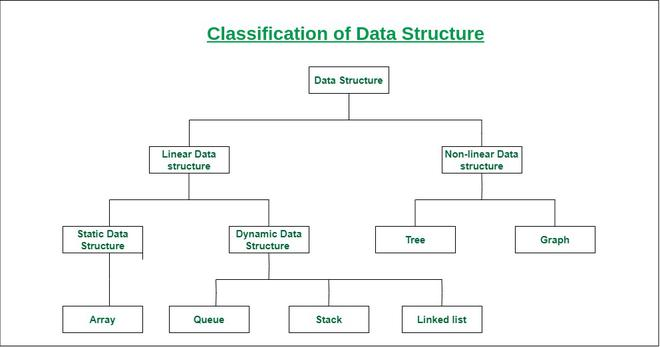
\includegraphics[width=0.5\linewidth,height=6cm,keepaspectratio]{Pictures/ds-algo/ClassificationofDataStructures.jpg}
    \caption{Types of Data Structure}
\end{figure}

\subsection{Linear Data Structure \cite{gfg-data-structures}}
\begin{enumerate}
    \item Data structure in which data elements are arranged sequentially or linearly, where each element is attached to its previous and next adjacent elements, is called a linear data structure.
    
    \item \textbf{Example}: Array, Stack, Queue, Linked List, etc.
\end{enumerate}

\subsection{Static Data Structure \cite{gfg-data-structures}}
\begin{enumerate}
    \item Static data structure has a fixed memory size. It is easier to access the elements in a static data structure. 

    \item \textbf{Example}: array.
\end{enumerate}

\subsection{Dynamic Data Structure \cite{gfg-data-structures}}
\begin{enumerate}
    \item In dynamic data structure, the size is not fixed. It can be randomly updated during the runtime which may be considered efficient concerning the memory (space) complexity of the code.

    \item \textbf{Example}: Queue, Stack, etc.
\end{enumerate}

\subsection{Non-Linear Data Structure \cite{gfg-data-structures}}
\begin{enumerate}
    \item Data structures where data elements are not placed sequentially or linearly are called non-linear data structures. In a non-linear data structure, we can’t traverse all the elements in a single run only.
    
    \item \textbf{Example}: Trees and Graphs.
\end{enumerate}

\section{Array \cite{gfg-array-data-structure-guide}}\label{array}

\begin{table}[h]
    \begin{minipage}{0.35\linewidth}
        \begin{figure}[H]
            \centering
            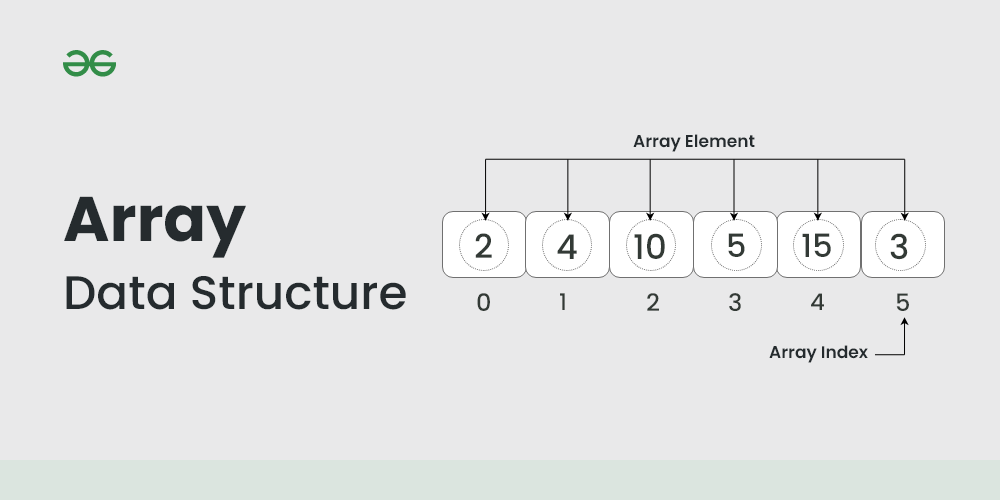
\includegraphics[width=\linewidth,height=5cm,keepaspectratio]{Pictures/ds-algo/Array-data-structure.png}
            \caption{Data Structure: Array}
        \end{figure}
    \end{minipage}
    \hfill
    \begin{minipage}{0.65\linewidth}
        \begin{enumerate}
            \item An array data structure is a fundamental concept in computer science that stores a collection of elements in a contiguous block of memory.

            \item It allows for efficient access to elements using indices and is widely used in programming for organizing and manipulating data.

            \item Each item in an array is indexed starting with $\mathbf{0}$. 
            
            \item Each element in an array is accessed through its index.
        \end{enumerate}
    \end{minipage}
\end{table}

\noindent \textbf{Types of Array}
\begin{enumerate}
    \item \textbf{One-dimensional arrays}: These arrays store a single row of elements.
    \item \textbf{Multidimensional arrays}: These arrays store multiple rows of elements.
\end{enumerate}

\subsection{Array Operations}
\begin{enumerate}
    \item \fullref{Linear Search Algorithm}
    \item \fullref{Binary Search Algorithm}
    \item \fullref{Ternary Search}
    \item \fullref{Exponential Search}
\end{enumerate}









































